\documentclass{article}\usepackage[]{graphicx}\usepackage[]{color}
%% maxwidth is the original width if it is less than linewidth
%% otherwise use linewidth (to make sure the graphics do not exceed the margin)
\makeatletter
\def\maxwidth{ %
  \ifdim\Gin@nat@width>\linewidth
    \linewidth
  \else
    \Gin@nat@width
  \fi
}
\makeatother

\definecolor{fgcolor}{rgb}{0.345, 0.345, 0.345}
\newcommand{\hlnum}[1]{\textcolor[rgb]{0.686,0.059,0.569}{#1}}%
\newcommand{\hlstr}[1]{\textcolor[rgb]{0.192,0.494,0.8}{#1}}%
\newcommand{\hlcom}[1]{\textcolor[rgb]{0.678,0.584,0.686}{\textit{#1}}}%
\newcommand{\hlopt}[1]{\textcolor[rgb]{0,0,0}{#1}}%
\newcommand{\hlstd}[1]{\textcolor[rgb]{0.345,0.345,0.345}{#1}}%
\newcommand{\hlkwa}[1]{\textcolor[rgb]{0.161,0.373,0.58}{\textbf{#1}}}%
\newcommand{\hlkwb}[1]{\textcolor[rgb]{0.69,0.353,0.396}{#1}}%
\newcommand{\hlkwc}[1]{\textcolor[rgb]{0.333,0.667,0.333}{#1}}%
\newcommand{\hlkwd}[1]{\textcolor[rgb]{0.737,0.353,0.396}{\textbf{#1}}}%
\let\hlipl\hlkwb

\usepackage{framed}
\makeatletter
\newenvironment{kframe}{%
 \def\at@end@of@kframe{}%
 \ifinner\ifhmode%
  \def\at@end@of@kframe{\end{minipage}}%
  \begin{minipage}{\columnwidth}%
 \fi\fi%
 \def\FrameCommand##1{\hskip\@totalleftmargin \hskip-\fboxsep
 \colorbox{shadecolor}{##1}\hskip-\fboxsep
     % There is no \\@totalrightmargin, so:
     \hskip-\linewidth \hskip-\@totalleftmargin \hskip\columnwidth}%
 \MakeFramed {\advance\hsize-\width
   \@totalleftmargin\z@ \linewidth\hsize
   \@setminipage}}%
 {\par\unskip\endMakeFramed%
 \at@end@of@kframe}
\makeatother

\definecolor{shadecolor}{rgb}{.97, .97, .97}
\definecolor{messagecolor}{rgb}{0, 0, 0}
\definecolor{warningcolor}{rgb}{1, 0, 1}
\definecolor{errorcolor}{rgb}{1, 0, 0}
\newenvironment{knitrout}{}{} % an empty environment to be redefined in TeX

\usepackage{alltt}
\IfFileExists{upquote.sty}{\usepackage{upquote}}{}
\begin{document}

\begin{knitrout}
\definecolor{shadecolor}{rgb}{0.969, 0.969, 0.969}\color{fgcolor}\begin{kframe}
\begin{alltt}
\hlcom{# Strategy of safe distr. of <U>|[V]}
\hlstd{MontyHallU} \hlkwb{<-} \hlkwa{function} \hlstd{() \{}
  \hlcom{# Count the correct guesses when door 2 is opened}
  \hlstd{U2} \hlkwb{=} \hlkwd{sample}\hlstd{(}\hlkwd{c}\hlstd{(}\hlnum{1}\hlstd{,}\hlnum{3}\hlstd{), twos,} \hlkwc{replace} \hlstd{=} \hlnum{TRUE}\hlstd{)}
  \hlstd{hit} \hlkwb{=} \hlkwd{sum}\hlstd{(U2} \hlopt{==} \hlstd{setup[setup[,}\hlnum{2}\hlstd{]} \hlopt{==} \hlnum{2}\hlstd{][}\hlnum{1}\hlopt{:}\hlstd{twos])}

  \hlcom{# Count the correct guesses when door 3 is opened}
  \hlstd{hit} \hlkwb{=} \hlstd{hit} \hlopt{+} \hlkwd{sum}\hlstd{(}\hlnum{2} \hlopt{==} \hlstd{setup[setup[,}\hlnum{2}\hlstd{]} \hlopt{==} \hlnum{3}\hlstd{][}\hlnum{1}\hlopt{:}\hlstd{threes])}

  \hlstd{hit}\hlopt{/}\hlstd{N}
\hlstd{\}}

\hlcom{# Strategy of safe distr. of 1_\{U=1\}|[V]}
\hlstd{MontyHall1U} \hlkwb{<-} \hlkwa{function}\hlstd{() \{}
  \hlcom{# Count the correct guesses when door 2 is opened}
  \hlstd{U2} \hlkwb{=} \hlkwd{sample}\hlstd{(}\hlkwd{c}\hlstd{(}\hlnum{1}\hlstd{,}\hlnum{3}\hlstd{), twos,} \hlkwc{replace} \hlstd{=} \hlnum{TRUE}\hlstd{,} \hlkwc{prob} \hlstd{=} \hlkwd{c}\hlstd{(}\hlnum{1}\hlopt{/}\hlnum{3}\hlstd{,}\hlnum{2}\hlopt{/}\hlnum{3}\hlstd{))}
  \hlstd{hit} \hlkwb{=} \hlkwd{sum}\hlstd{(U2} \hlopt{==} \hlstd{setup[setup[,}\hlnum{2}\hlstd{]} \hlopt{==} \hlnum{2}\hlstd{][}\hlnum{1}\hlopt{:}\hlstd{twos])}

  \hlcom{# Count the correct guesses when door 3 is opened}
  \hlstd{U3} \hlkwb{=} \hlkwd{sample}\hlstd{(}\hlkwd{c}\hlstd{(}\hlnum{1}\hlstd{,}\hlnum{2}\hlstd{), threes,} \hlkwc{replace} \hlstd{=} \hlnum{TRUE}\hlstd{,} \hlkwc{prob} \hlstd{=} \hlkwd{c}\hlstd{(}\hlnum{1}\hlopt{/}\hlnum{3}\hlstd{,}\hlnum{2}\hlopt{/}\hlnum{3}\hlstd{))}
  \hlstd{hit} \hlkwb{=} \hlstd{hit} \hlopt{+} \hlkwd{sum}\hlstd{(U3} \hlopt{==} \hlstd{setup[setup[,}\hlnum{2}\hlstd{]} \hlopt{==} \hlnum{3}\hlstd{][}\hlnum{1}\hlopt{:}\hlstd{threes])}

  \hlstd{hit}\hlopt{/}\hlstd{N}
\hlstd{\}}

\hlcom{# Strategy of optimal distribution of always switch}
\hlstd{MontyHallMax} \hlkwb{<-} \hlkwa{function}\hlstd{() \{}
  \hlcom{# Count the correct guesses when door 2 is opened}
  \hlstd{U2} \hlkwb{=} \hlkwd{sample}\hlstd{(}\hlkwd{c}\hlstd{(}\hlnum{1}\hlstd{,}\hlnum{3}\hlstd{), twos,} \hlkwc{replace} \hlstd{=} \hlnum{TRUE}\hlstd{,} \hlkwc{prob} \hlstd{=} \hlkwd{c}\hlstd{(}\hlnum{0}\hlstd{,}\hlnum{1}\hlstd{))}
  \hlstd{hit} \hlkwb{=} \hlkwd{sum}\hlstd{(U2} \hlopt{==} \hlstd{setup[setup[,}\hlnum{2}\hlstd{]} \hlopt{==} \hlnum{2}\hlstd{][}\hlnum{1}\hlopt{:}\hlstd{twos])}

  \hlcom{# Count the correct guesses when door 3 is opened}
  \hlstd{U3} \hlkwb{=} \hlkwd{sample}\hlstd{(}\hlkwd{c}\hlstd{(}\hlnum{1}\hlstd{,}\hlnum{2}\hlstd{), threes,} \hlkwc{replace} \hlstd{=} \hlnum{TRUE}\hlstd{,} \hlkwc{prob} \hlstd{=} \hlkwd{c}\hlstd{(}\hlnum{0}\hlstd{,}\hlnum{1}\hlstd{))}
  \hlstd{hit} \hlkwb{=} \hlstd{hit} \hlopt{+} \hlkwd{sum}\hlstd{(U3} \hlopt{==} \hlstd{setup[setup[,}\hlnum{2}\hlstd{]} \hlopt{==} \hlnum{3}\hlstd{][}\hlnum{1}\hlopt{:}\hlstd{threes])}

  \hlstd{hit}\hlopt{/}\hlstd{N}
\hlstd{\}}

\hlstd{doors} \hlkwb{=} \hlkwd{list}\hlstd{(}\hlkwd{c}\hlstd{(}\hlnum{1}\hlstd{,}\hlnum{2}\hlstd{),} \hlkwd{c}\hlstd{(}\hlnum{1}\hlstd{,}\hlnum{3}\hlstd{),} \hlkwd{c}\hlstd{(}\hlnum{2}\hlstd{,}\hlnum{3}\hlstd{),} \hlkwd{c}\hlstd{(}\hlnum{3}\hlstd{,}\hlnum{2}\hlstd{))}
\hlstd{N} \hlkwb{=} \hlnum{10000} \hlcom{# Amount of Monty Hall games per q}
\hlstd{dt} \hlkwb{=} \hlnum{0.01} \hlcom{# Step size of q}

\hlstd{gamesU} \hlkwb{=} \hlkwd{vector}\hlstd{(}\hlkwc{length}\hlstd{=}\hlnum{1}\hlopt{/}\hlstd{dt}\hlopt{+}\hlnum{1}\hlstd{)}
\hlstd{games1U} \hlkwb{=} \hlkwd{vector}\hlstd{(}\hlkwc{length}\hlstd{=}\hlnum{1}\hlopt{/}\hlstd{dt}\hlopt{+}\hlnum{1}\hlstd{)}
\hlstd{gamesMax} \hlkwb{=} \hlkwd{vector}\hlstd{(}\hlkwc{length}\hlstd{=}\hlnum{1}\hlopt{/}\hlstd{dt}\hlopt{+}\hlnum{1}\hlstd{)}

\hlkwa{for} \hlstd{(i} \hlkwa{in} \hlnum{1}\hlopt{:}\hlstd{(}\hlnum{1}\hlopt{/}\hlstd{dt}\hlopt{+}\hlnum{1}\hlstd{)) \{}
  \hlcom{# Update Monty Hall's strategy}
  \hlstd{chances} \hlkwb{=} \hlkwd{c}\hlstd{((i}\hlopt{-}\hlnum{1}\hlstd{)}\hlopt{*}\hlstd{dt}\hlopt{/}\hlnum{3}\hlstd{, (}\hlnum{1}\hlopt{-}\hlstd{(i}\hlopt{-}\hlnum{1}\hlstd{)}\hlopt{*}\hlstd{dt)}\hlopt{/}\hlnum{3}\hlstd{,} \hlnum{1}\hlopt{/}\hlnum{3}\hlstd{,} \hlnum{1}\hlopt{/}\hlnum{3}\hlstd{)}
  \hlcom{# Place the car and open a door N times}
  \hlstd{setup} \hlkwb{=} \hlkwd{matrix}\hlstd{(}\hlkwd{unlist}\hlstd{(}\hlkwd{sample}\hlstd{(doors, N,} \hlnum{TRUE}\hlstd{, chances)),}
                 \hlkwc{ncol} \hlstd{=} \hlnum{2}\hlstd{,} \hlkwc{byrow} \hlstd{=} \hlnum{TRUE}\hlstd{)}
  \hlcom{# Count the number of times door 2 is opened}
  \hlstd{twos} \hlkwb{=} \hlkwd{length}\hlstd{(}\hlkwd{which}\hlstd{(setup[,}\hlnum{2}\hlstd{]} \hlopt{==} \hlnum{2}\hlstd{))}
  \hlcom{# Count the number of times door 3 is opened}
  \hlstd{threes} \hlkwb{=} \hlkwd{length}\hlstd{(}\hlkwd{which}\hlstd{(setup[,}\hlnum{2}\hlstd{]} \hlopt{==} \hlnum{3}\hlstd{))}

  \hlcom{# Play safe strategy for <U>|[V]}
  \hlstd{gamesU[i]} \hlkwb{=} \hlkwd{MontyHallU}\hlstd{()}
  \hlcom{# Play safe strategy for 1_\{U=1\}|[V]}
  \hlstd{games1U[i]} \hlkwb{=} \hlkwd{MontyHall1U}\hlstd{()}
  \hlcom{# Play optimal strategy}
  \hlstd{gamesMax[i]} \hlkwb{=} \hlkwd{MontyHallMax}\hlstd{()}
\hlstd{\}}

\hlcom{####}
\hlcom{# Plot the hit percentages against q}
\hlkwd{plot}\hlstd{(}\hlkwd{seq}\hlstd{(}\hlnum{0}\hlstd{,}\hlnum{1}\hlstd{,dt), gamesU,} \hlkwc{col}\hlstd{=}\hlstr{'blue'}\hlstd{,} \hlkwc{xlab}\hlstd{=}\hlstr{"q"}\hlstd{,}
     \hlkwc{ylab}\hlstd{=}\hlstr{"Percentage of correct guesses"}\hlstd{,}
     \hlkwc{main}\hlstd{=}\hlstr{"Percentage of correct guesses against q"}\hlstd{)}
\hlkwd{points}\hlstd{(}\hlkwd{seq}\hlstd{(}\hlnum{0}\hlstd{,}\hlnum{1}\hlstd{,dt), games1U,} \hlkwc{pch}\hlstd{=}\hlnum{4}\hlstd{,} \hlkwc{col}\hlstd{=}\hlstr{'red'}\hlstd{)}
\hlkwd{points}\hlstd{(}\hlkwd{seq}\hlstd{(}\hlnum{0}\hlstd{,}\hlnum{1}\hlstd{,dt), gamesMax,} \hlkwc{pch}\hlstd{=}\hlnum{5}\hlstd{,} \hlkwc{col}\hlstd{=}\hlstr{'orange'}\hlstd{)}
\hlkwd{abline}\hlstd{(}\hlkwc{h}\hlstd{=}\hlnum{5}\hlopt{/}\hlnum{9}\hlstd{,} \hlkwc{col}\hlstd{=}\hlstr{'red'}\hlstd{)}
\hlkwd{abline}\hlstd{(}\hlnum{1}\hlopt{/}\hlnum{2}\hlstd{,}\hlnum{1}\hlopt{/}\hlnum{6}\hlstd{,} \hlkwc{col}\hlstd{=}\hlstr{'blue'}\hlstd{)}
\hlkwd{abline}\hlstd{(}\hlkwc{h}\hlstd{=}\hlnum{2}\hlopt{/}\hlnum{3}\hlstd{,} \hlkwc{col}\hlstd{=}\hlstr{'orange'}\hlstd{)}
\end{alltt}
\end{kframe}
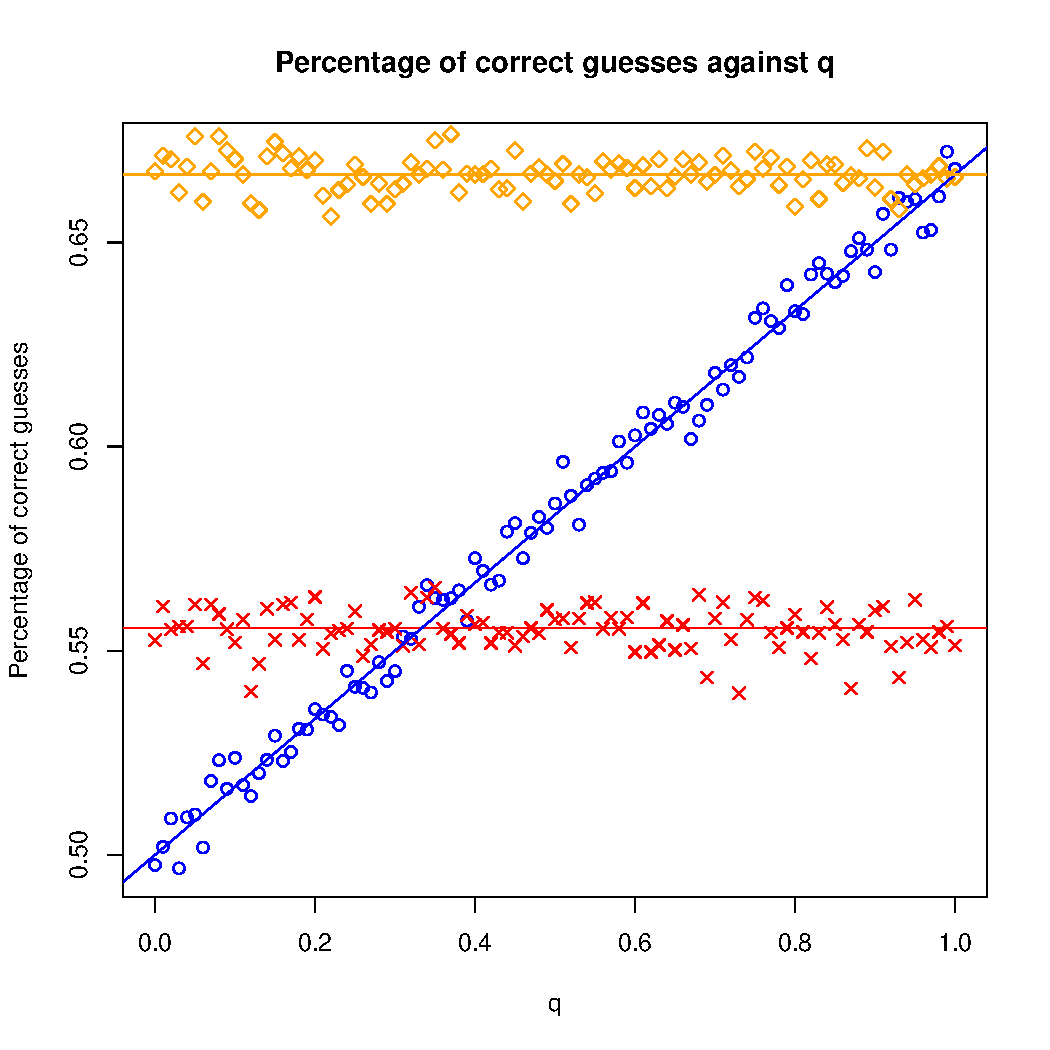
\includegraphics[width=\maxwidth]{figure/unnamed-chunk-1-1} 

\end{knitrout}


\end{document}
